\section{Resultater}

\subsection{}
\begin{figure}[h]
\centering
\begin{center}
    \emph{Hvilken kjønn er du?}
\end{center}
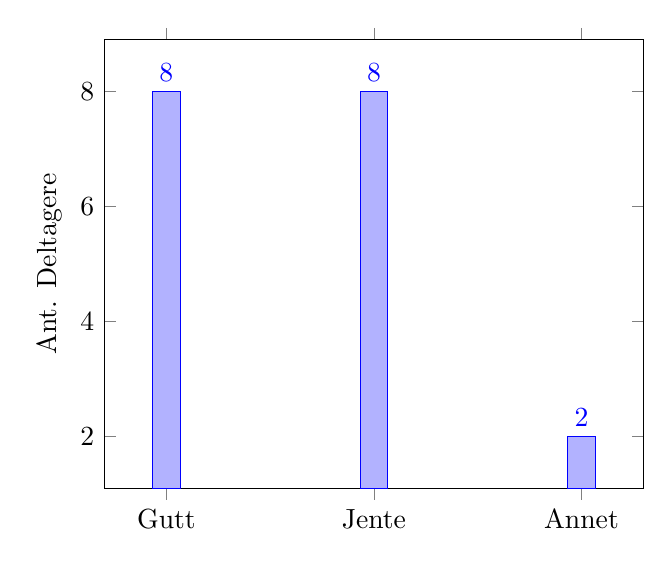
\begin{tikzpicture}
    \begin{axis}[ybar, enlargelimits=0.15, legend style={at={(0.5,-0.2)},
        anchor=north, legend columns=-1}, ylabel={Ant. Deltagere},
        symbolic x coords={Gutt, Jente, Annet}, xtick=data,
        nodes near coords, nodes near coords align={vertical},]
        % x tick label style={rotate=15, anchor=east},
        \addplot coordinates {(Gutt, 8) (Jente, 8) (Annet, 2)};
    \end{axis}
\end{tikzpicture}
\caption{Test}
\end{figure}
    
\newpage